\documentclass[a4paper,12pt]{article}
\usepackage[utf8]{inputenc}
\usepackage[T1]{fontenc}
\usepackage[french]{babel}
\usepackage[right=2.5cm, left=2.5cm]{geometry}
\usepackage[ddmmyyyy]{datetime}
\usepackage[table]{xcolor}
\usepackage{lmodern,mathptmx,changepage,titlesec,hyperref,listings,lstautogobble,graphicx,array,longtable,multirow,lipsum,tikz,shorttoc,enumitem}
\usetikzlibrary{arrows,automata}
\usetikzlibrary{positioning}

\renewcommand{\rmdefault}{\sfdefault} %Utilisation de la police sans-serif ("Computer Modern Sans") pour la police roman
\renewcommand{\ttdefault}{pcr} 	%Utilisation d'une police "CourrierNew" pour la police monospaced (pour faire un listing manuel)
\linespread{1.15}				%Interligne

%Utilisation de liens colorés en bleu et soulignés
\hypersetup{colorlinks=true, urlcolor=blue, urlbordercolor=blue, linkcolor=black, linkbordercolor=white}
\makeatletter \Hy@AtBeginDocument{\def\@pdfborder{0 0 1} \def\@pdfborderstyle{/S/U/W 1}}\makeatother

\titlespacing*{\section} {0cm}{7ex plus 1ex minus .2ex}{1.5ex plus .2ex}
\titlespacing*{\subsection} {0cm}{4.5ex plus 1ex minus .2ex}{1.5ex plus .2ex}
\titleformat*{\section}{\huge\bfseries}
\titleformat*{\subsection}{\Large\bfseries}
\titleformat*{\subsubsection}{\normalsize\bfseries}

\definecolor{darkgreen}{rgb}{0,0.8,0}
\definecolor{mygray}{rgb}{0.93,0.93,0.93}
\definecolor{mymauve}{rgb}{0.58,0,0.82}
\lstset{	
	basicstyle=\small\ttfamily,
	backgroundcolor=\color{mygray},
	breaklines=true,
	breakatwhitespace=true,
	postbreak=\raisebox{0ex}[0ex][0ex]{\ensuremath{\color{red}\hookrightarrow\space}},
	tabsize=3,
	frame=none,
	rulecolor=\color{black},
	keywordstyle=\color{blue}\bfseries,
	stringstyle=\color{orange},
	showstringspaces=false,
	commentstyle=\footnotesize\color{darkgreen},
	keepspaces=true,
	extendedchars=true,
	numbers=left,
	numberstyle=\tiny\color{lightgray},
	stepnumber=1,
	escapeinside={(@}{@)},
	autogobble=true,
	literate=
		{á}{{\'a}}1 {é}{{\'e}}1 {í}{{}}1 {ó}{{\'o}}1 {ú}{{\'u}}1
		{Á}{{\'A}}1 {É}{{\'E}}1 {Í}{{\'I}}1 {Ó}{{\'O}}1 {Ú}{{\'U}}1
		{à}{{\`a}}1 {è}{{\`e}}1 {ì}{{\`i}}1 {ò}{{\`o}}1 {ù}{{\`u}}1
		{À}{{\`A}}1 {È}{{\'E}}1 {Ì}{{\`I}}1 {Ò}{{\`O}}1 {Ù}{{\`U}}1
		{ä}{{\"a}}1 {ë}{{\"e}}1 {ï}{{\"i}}1 {ö}{{\"o}}1 {ü}{{\"u}}1
		{Ä}{{\"A}}1 {Ë}{{\"E}}1 {Ï}{{\"I}}1 {Ö}{{\"O}}1 {Ü}{{\"U}}1
		{â}{{\^a}}1 {ê}{{\^e}}1 {î}{{\^i}}1 {ô}{{\^o}}1 {û}{{\^u}}1
		{Â}{{\^A}}1 {Ê}{{\^E}}1 {Î}{{\^I}}1 {Ô}{{\^O}}1 {Û}{{\^U}}1
		{œ}{{\oe}}1 {Œ}{{\OE}}1 {æ}{{\ae}}1 {Æ}{{\AE}}1 {ß}{{\ss}}1
		{ç}{{\c c}}1 {Ç}{{\c C}}1 {ø}{{\o}}1 {å}{{\r a}}1 {Å}{{\r A}}1
		{€}{{e}}1 {£}{{\pounds}}1 {«}{{\guillemotleft}}1
		{»}{{\guillemotright}}1 {ñ}{{\~n}}1 {Ñ}{{\~N}}1 {¿}{{?`}}1
}

%Redéfinition de la taille de \Huge pour le titre du document
\makeatletter\renewcommand\Huge{\@setfontsize\Huge{37pt}{40}}\makeatother
\date{\today}

\title{\vspace{\fill}\textbf{\Huge Spécifications}}
\author{
	Sonny Klotz - Jean-Didier Pailleux - Malek Zemni
	\vspace{2em}\\
	\textit{Interface de chargement, de contrôle}\\\textit{et d’analyse statistique des données}\\\textit{pour la constitution d’un graphe de flux}
	\vspace{2em}
}

\begin{document}
\pagenumbering{gobble}\clearpage
\maketitle\vspace{8em}
\begin{center}
\includegraphics[scale=0.7]{../Cahier/logo.png}\end{center}
\begin{flushright}Module \textit{Projet}\end{flushright}
\newpage
\tableofcontents
\newpage\clearpage\pagenumbering{arabic}

	\section*{Introduction}
		Ce document va décrire l'ensemble des exigences fonctionnelles que doit satisfaire notre produit final, c'est-à-dire les différentes fonctionnalités que notre application va fournir. Cette description va prendre en compte les caractéristiques des outils de développement choisis.
		\paragraph{}Notre outil, Python, est un langage de programmation hybride alliant programmation fonctionnelle et objet. Dans Python, le type de données n'est connu qu'à l'exécution (typage dynamique), par conséquent, ces types ne seront pas indiqués dans les signatures des fonctionnalités. Ils seront précisés dans des paragraphes explicatifs.
		\paragraph{}Pour les parties qui s'appuient sur une interaction avec l'utilisateur, notre démarche de description des fonctionnalités va essentiellement prendre en compte l'\textit{expérience utilisateur}\footnote{http://uxdesign.com/ux-defined}. Cette description sera donc axée sur la qualification du résultat et du ressenti de l'utilisateur lors de la manipulation de l'interface fournie (une illustration à l'aide de croquis), plutôt que sur les points techniques de l'application (fonctions et classes).
		\paragraph{}Les fonctionnalités de notre application seront présentées selon les modules de l'organigramme établi dans le cahier des charges. Ces modules eux-mêmes seront regroupés en packages. Ce document va donc décrire, pour chaque package de l'organigramme, les fonctionnalités de ses modules : d'abord ceux du package de chargement des données, ensuite ceux du package d'analyse descriptive des données et enfin ceux du package de l'interface web. Dans une dernière partie, un glossaire sera consacré à la définition des types de données utilisés.
		
	\section{Package Chargement des données}
	Ce package est composé de 2 modules qui ont pour fonction de traiter le fichier de données fourni : une vérification de son format et une analyse de son contenu.
		
		\subsection{Module Vérification format fichier}
			Ce module va vérifier le format du fichier de données fourni en entrée en 3 points. Il aura donc 3 fonctionnalités de vérification et une fonctionnalité globale d'ouverture du fichier.
			\begin{enumerate}
				\vspace{1em}\item Fonctionnalité de vérification de l'ouverture du fichier :
					\begin{lstlisting}
						verifOuverture(fichierCSV)
					\end{lstlisting}
					\underline{Paramètres :}
						\begin{description}[style=unboxed,leftmargin=0.2cm]
							\item\lstinline!fichierCSV! : \lstinline!TextIoWrapper! - représente le fichier CSV fourni.
						\end{description}
					\underline{Retour :} variable de type entier signalant un succès (0) ou une erreur (1).\\
					\underline{Description :} cette fonction prend en entrée le fichier CSV ouvert. Elle vérifie que le paramètre \lstinline!fichierCSV! contient bien des informations représentant un fichier quelconque, et renvoie l'entier 0 si c'est le cas, l'entier 1 sinon.
				\vspace{1em}\item Fonctionnalité de vérification de l'extension du fichier ouvert :
					\begin{lstlisting}
						verifExtenstion(fichierCSV)
					\end{lstlisting}
					\underline{Paramètres :}
						\begin{description}[style=unboxed,leftmargin=0.2cm]
							\item\lstinline!fichierCSV! : \lstinline!TextIoWrapper! - représente le fichier CSV fourni.
						\end{description}
					\underline{Retour :} variable de type entier signalant un succès (0) ou une erreur (2).\\
					\underline{Description :} cette fonction prend en entrée le fichier CSV ouvert. Elle vérifie que l'information décrivant l'extension du fichier dans le paramètre \lstinline!fichierCSV! correspond bien au format CSV, et renvoie l'entier 0 si c'est le cas, l'entier 2 sinon.
				\vspace{1em}\item Fonctionnalité de vérification de l'accessibilité en lecture du fichier :
					\begin{lstlisting}
						verifLecture(fichierCSV)
					\end{lstlisting}
					\underline{Paramètres :}
						\begin{description}[style=unboxed,leftmargin=0.2cm]
							\item\lstinline!fichierCSV! : \lstinline!TextIoWrapper! - représente le fichier CSV fourni.
						\end{description}
					\underline{Retour :} variable de type entier signalant un succès (0) ou une erreur (3).\\
					\underline{Description :} cette fonction prend en entrée le fichier CSV ouvert. Elle vérifie que le paramètre \lstinline!fichierCSV! représentant le fichier possède bien la propriété d'accès en lecture. Un test de lecture sera aussi effectué sur le fichier. La fonction renvoie l'entier 0 si l'accès en lecture est permis, l'entier 3 sinon.
				\vspace{1em}\item Fonctionnalité globale d'ouverture du fichier CSV :
					\begin{lstlisting}
						ouvrir(chemin)
					\end{lstlisting}
					\underline{Paramètres :}
						\begin{description}[style=unboxed,leftmargin=0.2cm]
							\item\lstinline!chemin! : \lstinline!str! - chaîne de caractères représentant le chemin relatif ou absolu du fichier CSV fourni.
						\end{description}
					\underline{Retour :} variable de type chaîne de caractères signalant le succès ou la description d'une erreur.\\
					\underline{Description :} cette fonction prend en entrée le chemin du fichier CSV fourni. Elle ouvre ce fichier en lecture à l'aide de la fonction \lstinline!open(chemin,"r")! et le stocke dans une variable de type \lstinline!TextIoWrapper!. Elle applique ensuite dans l'ordre les trois fonctions de vérifications du module et renvoie la description de la fonction qui fait échouer l'ouverture (texte correspondant au code 1, 2 ou 3), ou bien la chaîne \lstinline!"success"! signalant le succès de l'ouverture.
			\end{enumerate}
		
		
		\subsection{Module Analyse contenu fichier}
			Ce module va analyser le contenu du fichier fourni en lisant une à une les données de ce fichier et en repérant les données erronées. Il aura donc 2 fonctionnalités :
			\begin{enumerate}
				\vspace{1em}\item Fonctionnalité de lecture du contenu du fichier CSV :
					\begin{lstlisting}
						lecture(fichierCSV)
					\end{lstlisting}
					\underline{Paramètres :}
						\begin{description}[style=unboxed,leftmargin=0.2cm]
							\item\lstinline!fichierCSV! : \lstinline!TextIoWrapper! - représente le fichier CSV fourni.
						\end{description}
					\underline{Retour :} une variable de type \lstinline!list! : une liste dont chaque élément est une sous-liste contenant les données d'une ligne du fichier CSV.\\
					\underline{Description :} cette fonction prend en entrée le fichier CSV ouvert. Elle crée une liste pour y sauvegarder le contenu de ce fichier, ligne par ligne. Elle lit les caractères du fichier en entier à l'aide de la fonction \lstinline!read()!. Ensuite, pour chaque ligne du fichier, elle applique la fonction \lstinline!split(',')! pour séparer les caractères de cette ligne selon la virgule et les stocker dans une sous-liste qui sera finalement stockée dans la liste englobante. L'utilisation d'une liste de listes permet d'indexer les lignes et les colonnes du fichier par leurs numéros.
					\begin{lstlisting}
						#Exemple d'un fichier CSV de 2 lignes à 2 données
						[ 	
							[donnéeColonne1Ligne1, donnéeColonne2Ligne1],
							[donnéeColonne1Ligne2, donnéeColonne2Ligne2]
						] 
					\end{lstlisting}
					
				\vspace{1em}\item Fonctionnalité de description du nom, du type et des erreurs des colonnes du fichier CSV :
					\begin{lstlisting}
						descriptionColonnes(lignesCSV)
					\end{lstlisting}
					\underline{Paramètres :}
						\begin{description}[style=unboxed,leftmargin=0.2cm]
							\item\lstinline!lignesCSV! : \lstinline!list! - liste représentant les données du fichier CSV ligne par ligne.
						\end{description}
					\underline{Retour :} une variable de type \lstinline!dict! : un dictionnaire de 3 sous-listes ayant pour clés : \lstinline!"nom"!, \lstinline!"type"! et \lstinline!"erreurs"!.\\
					\underline{Description :} cette fonction prend en entrée le fichier CSV préalablement lu et stocké dans la liste \lstinline!lignesCSV!. Elle crée un dictionnaire de 3 éléments de type liste, pour y renseigner le nom, le type et les lignes erronées de chaque colonne de ce fichier :\\
					1 - Elle remplit le champ \lstinline!"nom"! du dictionnaire par le nom de chaque colonne, lu à partir du fichier CSV.\\
					2 - Elle remplit le champ \lstinline!"type"! du dictionnaire par le type attendu pour chaque colonne.\\ 
					3 - Elle lit la liste \lstinline!lignesCSV! colonne par colonne. Pour chaque donnée d'une colonne, elle compare son type au type attendu et :\\
					\hspace*{1em} - en cas d'erreur, renseigne le descriptif de cette erreur dans la case correspondante à cette colonne dans une sous-sous-liste dans le champ \lstinline!"erreurs"! du dictionnaire,\\
					\hspace*{1em} - en cas de succès, inscrit la chaîne de caractères \lstinline!"correct"! dans la case correspondante de la sous-sous-liste du dictionnaire.\\
					\begin{lstlisting}
						#Exemple de description d'un fichier CSV de 2 lignes à 2 colonnes
						{ 	
							"nom" : ["nomColonne1", "nomColonne2"],
							"type" : [typeColonne1, typeColonne2],
							"erreurs" : 
							[
								["correct","description d'une erreur dans la colonne 2 de la ligne 1"], 
								["correct","correct"]
							] 
						} 
					\end{lstlisting}
					L'utilisation d'une telle structure pour le renseignement des erreurs permet un accès direct (indexé) lors de l'affichage des erreurs, et donc un gain de temps de calcul.
			\end{enumerate}
	
	\section{Package Analyse descriptive des données}
	Ce package est composé de trois modules d'ADD\footnote{ADD : analyse descriptive de données}. Ce package va aussi être livré au client pour une intégration externe. On pourra donc parler de API.
	
		\subsection{Module Analyse de données qualitatives}
			Ce module va effectuer les calculs d'effectifs, d'effectifs cumulés, de fréquences et de fréquences cumulées. Il s'occupera également de fournir les informations nécessaires pour la construction d'un diagramme en secteurs et d'un histogramme. Il aura donc 6 fonctionnalités :
	
			\begin{enumerate}
				\vspace{1em}\item Fonctionnalité de calcul de l'effectif :
					\begin{lstlisting}
						calculEffectifs(listeDonnees)
					\end{lstlisting}
					\underline{Paramètres :} 
					\begin{description}[style=unboxed,leftmargin=0.2cm]
						\item\lstinline!listeDonnees! : \lstinline!list! - structure contenant les données à analyser
					\end{description}
					\underline{Retour :} variable de type  \lstinline!list! : représente la sortie du calcul des effectifs de chaque valeur de la colonne.\\
					\underline{Description :} cette fonction prendra en paramètre une liste qui contiendra les données pour le calcul. Elle calculera les effectifs pour chaque valeur et effectuera un tri pour ordonner ces valeurs.
					
				\vspace{1em}\item Fonctionnalité de calcul des effectifs cumulés :
					\begin{lstlisting}
						calculEffectifsCumules(listeEffectifs)
					\end{lstlisting}
					\underline{Paramètres :} 
					\begin{description}[style=unboxed,leftmargin=0.2cm]
						\item\lstinline!listeEffectifs! : \lstinline!list! - correspond au résultat de la fonction \lstinline!calculEffectifs!.
					\end{description}
					\underline{Retour :} variable de type \lstinline!list! : copie du paramètre \lstinline!listeEffectifs! dont les effectifs seront remplacés par les effectifs cumulés.\\
					\underline{Description :} cette fonction prend en entrée les résultats de la fonction \lstinline!calculEffectifs! préalablement stocké dans une liste. Elle va copier dans une nouvelle liste celle rentrée en paramètre, et remplacera les effectifs par les effectifs cumulés. La fonction retournera cette nouvelle liste.
					
				\vspace{1em}\item Fonctionnalité pour calculer les fréquences d'apparition :
					\begin{lstlisting}
						calculFrequences(listeEffectifs)
					\end{lstlisting}
					\underline{Paramètres :} 
					\begin{description}[style=unboxed,leftmargin=0.2cm]
						\item\lstinline!listeEffectifs!  : \lstinline!list! - correspond au résultat de la fonction \lstinline!calculEffectifs!.
					\end{description}
					\underline{Retour :} variable de type \lstinline!list! : correspond à la sortie du calcul des fréquences de chaque valeur de la colonne.\\
					\underline{Description :} cette fonction prendra en paramètre une liste qui contiendra les données pour le calcul. Elle calculera les fréquences pour chaque valeur à partir de leur effectif.
					
				\vspace{1em}\item Fonctionnalité pour calculer les fréquences cumulées :
					\begin{lstlisting}
						calculFrequencesCumulees(listeEffectifsCumules)
					\end{lstlisting}
					\underline{Paramètres :} 
					\begin{description}[style=unboxed,leftmargin=0.2cm]
						\item\lstinline!listeEffectifsCumules! : \lstinline!list! - correspond au résultat de la fonction \lstinline!calculEffectifsCumules!.
					\end{description}
					\underline{Retour :} variable de type  \lstinline!list! - copie de \lstinline!listeEffectifsCumules! mais dont les effectifs seront divisés par le nombre d'élément total. \\
					\underline{Description :} cette fonction prend en entrée les résultats de la fonction \lstinline!calculEffectifsCumules! préalablement stockés dans une liste. Elle va copier dans une nouvelle liste celle rentrée en paramètre, et calculera les fréquences cumulées.
					
				\vspace{1em}\item Fonctionnalité fournissant les données du diagramme en secteurs :
					\begin{lstlisting}
						infoSecteurs(listeFrequences)
					\end{lstlisting}
					\underline{Paramètres :} 
					\begin{description}[style=unboxed,leftmargin=0.2cm]
						\item \lstinline!listeFrequences! :  \lstinline!list! - correspondant à la sortie du calcul des fréquences.
					\end{description}
					\underline{Retour :} sans retour (vide).\\
					\underline{Description :} cette fonction prend en entrée le résultat du calcul des fréquences préalablement stocké dans une liste \lstinline!listeFrequences!. Elle va créer un fichier \lstinline!.json! pour y stocker (écrire) les données nécessaires à la construction du diagramme en secteurs. Pour chaque couple (fréquence, valeur) elle va associer un angle compris entre 0\degre et 360\degre telle que la somme de tous les angles soit égale à 360\degre. Ne retourne aucune valeur.
					
				\vspace{1em}\item Fonctionnalité fournissant les données de l'histogramme :
					\begin{lstlisting}
						infoHistogramme(listeEffectifs)
					\end{lstlisting}
					\underline{Paramètres :} 
					\begin{description}[style=unboxed,leftmargin=0.2cm]
						\item \lstinline!listeEffectifs! : \lstinline!list! - correspond à la sortie du calcul des effectifs.
					\end{description}
					\underline{Retour :} sans retour (vide).\\
					\underline{Description :} cette fonction prend en entrée le résultat du calcul des effectifs préalablement stocké dans une liste \lstinline!listeEffectifs!. Elle va créer un fichier \lstinline!.json! pour y stocker (écrire) les données nécessaires à la construction de l'histogramme. Ne retourne aucune valeur.
			\end{enumerate}
		
		\subsection{Module Analyse de données quantitatives discrètes}
		
			\begin{enumerate}
				\vspace{1em}\item Calcul de la moyenne
					\begin{lstlisting}
						moyenne(listeEffectifs)
					\end{lstlisting}
					\underline{Paramètres :}
						\begin{description}[style=unboxed,leftmargin=0.2cm]
							\item \lstinline!listeEffectifs : list! - structure contenant les différents effectifs des données de l'ensemble analysé.
						\end{description}
					\underline{Type retour :} \lstinline!float! : moyenne arithmétique de l'ensemble de données\\
					\underline{Description :} Calcul de la moyenne arithmétique en fonction des données et de leur occurrences dans la liste.
				
				\vspace{1em}\item Calcul des quantiles (cas discret)
					\begin{lstlisting}
						quantileDiscret(ordre, listeFrequencesCumulees)
					\end{lstlisting}
					\underline{Paramètres :}
						\begin{description}[style=unboxed,leftmargin=0.2cm]
							\item \lstinline!ordre : float! - Nombre flottant compris entre 0 et 1
							\item \lstinline!listeFrequencesCumulees : list! - structure contenant les différentes fréquences cumulées des données de la colonne analysées
						\end{description}
					\underline{Type retour :} \lstinline!float!\\
					\underline{Description :} Valeur de la liste séparant les données en deux ensembles, le premier contenant la fraction \lstinline!ordre! des données, le deuxième contenant le reste. La médiane est le quantile d'ordre 1/2.
					
				\vspace{1em}\item Calcul de la variance
					\begin{lstlisting}
						variance(listeEffectifs)
					\end{lstlisting}
					\underline{Paramètres :}
						\begin{description}[style=unboxed,leftmargin=0.2cm]
							\item \lstinline!listeEffectif : list! - structure contenant les différents effectifs des données de l'ensemble analysé.
						\end{description}
					\underline{Type retour :} \lstinline!float!\\
					\underline{Description :} Variance de l'ensemble de données analysé.
				
				\vspace{1em}\item Calcul de l'écart-type
					\begin{lstlisting}
						ecartType(variance)
					\end{lstlisting}
					\underline{Paramètres :}
						\begin{description}[style=unboxed,leftmargin=0.2cm]
							\item \lstinline!variance : float!
						\end{description}
					\underline{Type retour :} \lstinline!float!\\
					\underline{Description :} Racine carrée de la variance.
					
				\vspace{1em}\item Détection des anomalies
					\begin{lstlisting}
						anomaliesTukey(listeEffectifs)
					\end{lstlisting}
					\underline{Paramètres :}
						\begin{description}[style=unboxed,leftmargin=0.2cm]
							\item \lstinline!listeEffectifs : list! - structure contenant les différents effectifs des données de l'ensemble analysé.
						\end{description}
					\underline{Type retour :}\lstinline!list! : collection contenant les données considérées anormales pour la distribution des valeurs\\
					\underline{Description :} Selon la méthode de Tukey, toute donnée n'étant pas contenue dans l'intervalle \lstinline![Q1 - 1.5*(Q3 - Q1) ; Q3 + 1.5*(Q3 - Q1)] !, avec \lstinline!Q1, Q3! les quartiles, est considérée comme une anomalie statistique.\footnote{https ://hal.archives-ouvertes.fr/halshs-00287751/document}
				
				\vspace{1em}\item Calcul du coefficient de symétrie
					\begin{lstlisting}
						symetrie(listeEffectifs)
					\end{lstlisting}
					\underline{Paramètres :}
						\begin{description}[style=unboxed,leftmargin=0.2cm]
							\item \lstinline!listeEffectifs : list! - structure contenant les différents effectifs des données de l'ensemble analysé.
						\end{description}
					\underline{Type retour :} \lstinline!float! - Nombre flottant compris entre -1 et 1.\\
					\underline{Description :} Coefficient d'asymétrie de Pearson calculé avec la moyenne, la médiane et l'écart-type: s'il est nul la distribution des valeurs est symétrique, s'il est positif, la série est étalée à droite, et s'il est négatif, la série est étalée  à gauche.
				
				\vspace{1em}\item Calcul du coefficient d'aplatissment
					\begin{lstlisting}
						aplatissement(listeEffectifs)
					\end{lstlisting} \lstinline!listeEffectifs : list! - structure contenant les différents effectifs des données de l'ensemble analysé.
					\underline{Paramètres :}
						\begin{description}[style=unboxed,leftmargin=0.2cm]
							\item
						\end{description}
					\underline{Type retour :}  \lstinline!float!\\
					\underline{Description :} Coefficient d'aplatissement de Fisher, calculé à partir de la moyenne et de l'écart-type. Si le coefficient est égal à 3, la série suit une loi normale centrée réduite, s'il est inférieur la distribution des valeurs est aplatie, et s'il est supérieur, les valeurs sont concentrées autour de la moyenne.
				
				\vspace{1em}\item Fonctionnalité pour les données de la distribution des valeurs (cas discret)
					\begin{lstlisting}
						infoDistributionDiscrete(listeEffectifs)
					\end{lstlisting}
					\underline{Paramètres :}
						\begin{description}[style=unboxed,leftmargin=0.2cm]
							\item \lstinline!listeEffectifs : list! - structure contenant les différents effectifs des données de l'ensemble analysé.
						\end{description}
					\underline{Retour :} aucun retour.\\
					\underline{Description :} Préparation de l'objet contenant les informations nécessaires à l'affichage de la distribution des valeurs (Diagramme en bâtons). Cette procédure écrit dans un fichier au format \lstinline!.json! pour stocker les couples (valeur, effectif) nécessaires au diagramme.
					
				\vspace{1em}\item Fonctionnalité pour les données de la distribution cumulative des valeurs (cas discret)
					\begin{lstlisting}
						infoDistributionCumulativeDiscrete(listeEffectifsCumules)
					\end{lstlisting}
					\underline{Paramètres :}
						\begin{description}[style=unboxed,leftmargin=0.2cm]
							\item \item \lstinline!listeEffectifsCumules : list! - structure contenant les différents effectifs cumulés des données de l'ensemble analysé.
						\end{description}
					\underline{Retour :} aucun retour.\\
					\underline{Description :} Préparation de l'objet contenant les informations nécessaires à l'affichage de la distribution cumulative des valeurs (diagramme en escaliers). Cette procédure écrit un fichier au format \lstinline!.json! - pour renseigner les couples (valeur, effectif cumulé).
					
				\vspace{1em}\item Fonctionnalité pour les données de la boîte à moustaches de Tukey
					\begin{lstlisting}
						infoBoiteTukey(listeEffectifs)
					\end{lstlisting}
					\underline{Paramètres :}
						\begin{description}[style=unboxed,leftmargin=0.2cm]
							\item \lstinline!listeEffectifs : list! - structure contenant les différents effectifs des données de l'ensemble analysé.
						\end{description}
					\underline{Retour :} aucun retour.\\
					\underline{Description :} La représentation graphique met en valeur les quartiles et la médiane, ainsi que les anomalies de Tukey. La procédure écrit un fichier fichier au format \lstinline!.csv! - contenant les données du paramètre. 
					
				\vspace{1em}\item Fonctionnalité pour les données de la série temporelle
					\begin{lstlisting}
						infoSerieTemporelle(listeSerieTemporelle)
					\end{lstlisting}
					\underline{Paramètres :}
						\begin{description}[style=unboxed,leftmargin=0.2cm]
							\item \lstinline!listeSerieTemporelle : list! - liste des couples (Timestamp, valeur) des données analysées.
						\end{description}
					\underline{Retour :} aucun retour.\\
					\underline{Description :} La représentation graphique associée consiste à afficher l'évolution des valeurs dans le temps. La procédure écrit un fichier au format \lstinline!.json! - contenant les couples (Timestamp, valeur).
			\end{enumerate}
			
		\subsection{Module Analyse de données quantitatives continues}
			\begin{enumerate}
				\vspace{1em}\item Fonctionnalité pour la discrétisation des valeurs
					\begin{lstlisting}
						discretisation(nombreClasses, donneesContinues)
					\end{lstlisting}
					\underline{Paramètres :}
						\begin{description}[style=unboxed,leftmargin=0.2cm]
							\item \lstinline!nombreClasses! : \lstinline!int! - indique en combien de classes d'intervalle l'étendue des données va être divisée.
							\item \lstinline!donnesContinues : list! - liste de flottants représentant les mesures analysées.
						\end{description}
					\underline{Type retour :} \lstinline!list! - collection d'\lstinline!Intervalle! (voir glossaire des types)\\
					\underline{Description :} La fonction se charge de décomposer l'étendue [min ; max] de l'ensemble de données en \lstinline!nombreClasses! intervalles de même étendue, puis de remplacer les occurrences des données par l'intervalle auquel la donnée appartient.
					
				\vspace{1em}\item Calcul du nombre de classes pour la discrétisation des valeurs
					\begin{lstlisting}
						calculNombreClasses(donneesContinues)
					\end{lstlisting}
					\underline{Paramètres :}
						\begin{description}[style=unboxed,leftmargin=0.2cm]
							\item \lstinline!donneesContinues : list! - liste de flottants représentant les mesures analysées.
						\end{description}
					\underline{Type retour :} \lstinline!int!\\
					\underline{Description :} Calcul le nombre de classes selon la règle de Sturges.
					
				\vspace{1em}\item Préparation des données pour l'utilisation des éléments de calcul du module ADD quantitatives discrètes
					\begin{lstlisting}
						preparationIntervallesAnalyse(listeIntervalles)
					\end{lstlisting}
					\underline{Paramètres :}
						\begin{description}[style=unboxed,leftmargin=0.2cm]
							\item \lstinline!listeIntervalles : list! - issue de la discrétisation des valeurs.
						\end{description}
					\underline{Type retour :} \lstinline!list! - liste de flottants\\
					\underline{Description :} Pour effectuer les analyses descriptives dans le cas continu, la démarche est la même (sauf quantiles) que pour le cas discret en utilisant comme données les centres des intervalles.
					
				\vspace{1em}\item Calcul des quantiles (cas continu)
					\begin{lstlisting}
						quantileContinu(ordre, listeFrequencesCumulees)
					\end{lstlisting}
					\underline{Paramètres :}
						\begin{description}[style=unboxed,leftmargin=0.2cm]
							\item \lstinline!ordre : float! - Nombre flottant compris entre 0 et 1
							\item \lstinline!listeFrequencesCumulees : list! - structure contenant les différentes fréquences cumulées des données de la colonne analysées
						\end{description}
					\underline{Type retour :} \lstinline!float!\\
					\underline{Description :} Les quantiles dans le cas continu sont calculés tout d'abord en identifiant la classe d'intervalle dans laquelle le quantile se trouve à l'aide des fréquences cumulées, puis par interpolation linéaire.
					
				\vspace{1em}\item Calcul d'abscisse par interpolation linéaire
					\begin{lstlisting}
						interpolationLineaire(p1, p2, y)
					\end{lstlisting}
					\underline{Paramètres :}
						\begin{description}[style=unboxed,leftmargin=0.2cm]
							\item \lstinline!p1 : float! Premier point de la droite
							\item \lstinline!p2 : float! Second point de la droite
							\item \lstinline!y : float! ordonnée du point dont on veut retrouver l'abscisse
						\end{description}
					\underline{Type retour :} \lstinline!float! - abscisse\\
					\underline{Description :} Les points  \lstinline!p1, p2! nous permettent d'identifier une fonction linéaire. On retrouve ensuite l'abscisse du point d'ordonnée  \lstinline!y! se trouvant sur la courbe de la fonction.
				
				\vspace{1em}\item Fonctionnalité pour les données de la distribution des valeurs (cas continu)
					\begin{lstlisting}
						infoDistributionContinue(listeEffectifs)
					\end{lstlisting}
					\underline{Paramètres :}
						\begin{description}[style=unboxed,leftmargin=0.2cm]
							\item \lstinline!listeEffectifs : list! - structure contenant les différents effectifs des données de l'ensemble analysé.
						\end{description}
					\underline{Retour :} aucun retour.\\
					\underline{Description :} Préparation de l'objet contenant les informations nécessaires à l'affichage de la distribution des valeurs. Cette procédure écrit dans un fichier au format \lstinline!.json! pour stocker les couples (valeur, effectif) nécessaires au diagramme.
					
				\vspace{1em}\item Fonctionnalité pour les données de la distribution cumulative des valeurs (cas continu)
					\begin{lstlisting}
						infoDistributionCumulativeContinue(listeFrequencesCumulees)
					\end{lstlisting}
					\underline{Paramètres :}
						\begin{description}[style=unboxed,leftmargin=0.2cm]
							\item \item \lstinline!listeFrequencesCumulees : list! - structure contenant les différentes fréquences cumulées des données de l'ensemble analysé.
						\end{description}
					\underline{Retour :} aucun retour.\\
					\underline{Description :} Préparation de l'objet contenant les informations nécessaires à l'affichage de la distribution cumulative des valeurs. La procédure écrit un fichier au format \lstinline!.json! - contenant les couples (valeur, fréquence cumulée).
					
			\end{enumerate}
		
	\section{Package Interface web}
		Ce package est composé de 3 modules de fenêtre graphique web qui assurent l'interaction avec l'utilisateur, et d'un module de gestion des flux qui s'occupe du lancement de l'application et de la transition des informations entre ses différents packages.
		
		\subsection{Module Gestion des flux}
		Ce module va lancer l'application et sera au centre du programme. Il s'occupera de gérer les branchements pour l'exécution, de faire transiter les informations entre les différents modules et de faire le traitement nécessaire en cas d'erreur. Il aura 4 fonctionnalités qui se chargeront de l'affichage des pages web dans lesquels les branchements seront gérés, ainsi que la fonctionnalité principale \lstinline!main! de l'application :
		
		\begin{enumerate} 
			\vspace{1em}\item Fonctionnalité principale de l'application :
				\begin{lstlisting}
					main()
				\end{lstlisting}
				\underline{Paramètres :}
					\begin{description}[style=unboxed,leftmargin=0.2cm]
						\item Ne prend aucun paramètre.
					\end{description}
				\underline{Retour :} sans retour (vide).\\
				\underline{Description :} cette fonction ne prend aucun paramètre en entrée et ne retourne rien en sortie. Elle s'occupe de lancer l'application en faisant appel à la première fenêtre choix fichier, et de gérer l'exécution du programme en fonction des commandes de l'utilisateur. Également la gestion des erreurs sera traité ainsi que l'arrêt du programme. 
				
			\vspace{1em}\item Fonctionnalité générant la fenêtre choix fichier :
				\begin{lstlisting}
					fenetre_choix_fichier()
				\end{lstlisting}
				\underline{Paramètres :}
					\begin{description}[style=unboxed,leftmargin=0.2cm]
						\item Ne prend aucun paramètre.
					\end{description}
				\underline{Retour :} \lstinline!render_template()! : fonction qui renvoie le contenu de la page web mis en paramètre qui va être envoyée à l'utilisateur.\\
				\underline{Description :} cette fonction correspond à la requête HTTP (c'est-à-dire le chemin de la page demandée) envoyée par le client (l'utilisateur) et reçue par le serveur qui sera soit un GET soit un POST. Pour cela il faudra indiquer avant de déclarer la fonction la ligne suivante : \lstinline!@app.route('/choix_fichier/', methods=['GET', 'POST'])!. Elle retournera le contenu de la page web mis en paramètre de la fonction \lstinline!render_template()! associé au code \lstinline!HTML! de la fenêtre choix fichier. Des variables en tant qu'arguments optionnels peuvent être utilisées dans le cas où l'on souhaiterait afficher des valeurs.
				
			\vspace{1em}\item Fonctionnalité générant la fenêtre rôle et choix colonne :
				\begin{lstlisting}
					fenetre_role_choix_colonne()
				\end{lstlisting}
				\underline{Paramètres :}
					\begin{description}[style=unboxed,leftmargin=0.2cm]
						\item Ne prend aucun paramètre.
					\end{description}
				\underline{Retour :} \lstinline!render_template()! : fonction qui renvoie le contenu de la page web mis en paramètre qui va être envoyée à l'utilisateur. \\
				\underline{Description :} cette fonction correspond à la requête HTTP (c'est à dire le chemin de la page demandée) envoyée par le client (l'utilisateur) et reçue par le serveur qui sera soit un GET soit un POST. Pour cela il faudra indiquer avant de déclarer la fonction la ligne suivante : \lstinline!@app.route('/role_choix_colonne/', methods=['GET', 'POST'])!. Elle retournera le contenu de la page web mis en paramètre de la fonction \lstinline!render_template()! associé au code \lstinline!HTML! de la fenêtre rôle et choix colonne. Des variables en tant qu'arguments optionnels peuvent être utilisées dans le cas où l'on souhaiterait afficher des valeurs.
				
			\vspace{1em}\item Fonctionnalité générant la fenêtre résultats ADD :
				\begin{lstlisting}
					fenetre_resultat_ADD()
				\end{lstlisting}
				\underline{Paramètres :}
					\begin{description}[style=unboxed,leftmargin=0.2cm]
						\item Ne prend aucun paramètre.
					\end{description}
				\underline{Retour :} \lstinline!render_template()! : fonction qui renvoie le contenu de la page web mis en paramètre qui va être envoyée à l'utilisateur. \\
				\underline{Description :} cette fonction correspond à la requête HTTP (c'est à dire le chemin de la page demandée) envoyée par le client (l'utilisateur) et reçue par le serveur qui sera soit un GET soit un POST. Pour cela il faudra indiquer avant de déclarer la fonction la ligne suivante : \lstinline!@app.route('/resultat_ADD/', methods=['GET', 'POST'])!. Elle retournera le contenu de la page web mis en paramètre de la fonction \lstinline!render_template()! associé au code \lstinline!HTML! de la fenêtre résultat ADD. Le deuxième argument qui sera mis dans \lstinline!render_template()! sera la liste contenant les données de la colonne choisie. Cette fonction sera appelé dès que le choix sera validé dans la fenêtre rôle et choix colonne pour accéder à la fenêtre suivante.
				
			\vspace{1em}\item Fonctionnalité de demande d'exportation :
				\begin{lstlisting}
					sauvegardeResultats()
				\end{lstlisting}
				\underline{Paramètres :}
					\begin{description}[style=unboxed,leftmargin=0.2cm]
						\item Ne prend aucun paramètre.
					\end{description}
				\underline{Retour :} sans retour (vide).\\
				\underline{Description :} cette fonction ne prend aucun paramètre. Elle s'active lorsque l'utilisateur fait la demande d'exporter les résultats depuis la fenêtre résultats ADD. Le téléchargement sera alors lancé par le navigateur web.
									
			\end{enumerate}
		
		\subsection{Module Fenêtre choix fichier}
		Ce module est une fenêtre graphique web qui permet à l'utilisateur de charger un fichier CSV. Ce module aura 2 fonctionnalités qui peuvent être illustrées par les croquis suivants :

			\begin{center}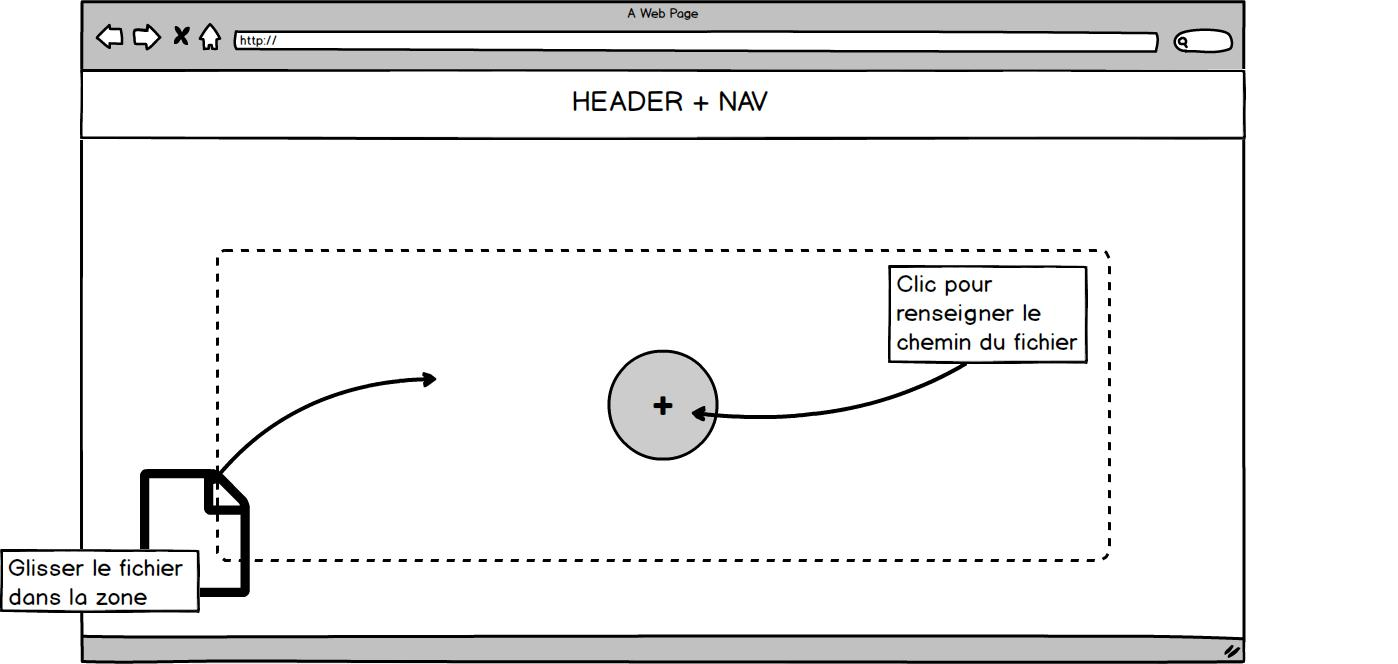
\includegraphics[scale=0.57]{Fenetre_choix_fichier1.jpg}\end{center} 
			\begin{center}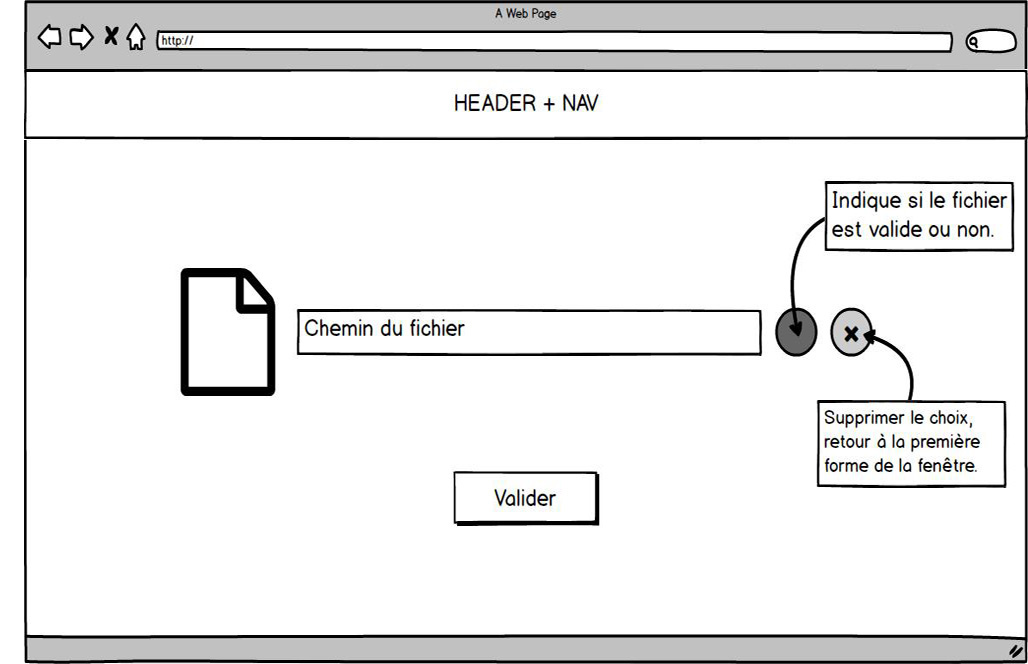
\includegraphics[scale=0.5]{Fenetre_choix_fichier2.jpg}\end{center}

			\begin{enumerate}
				\vspace{1em}\item Fonctionnalité d'ouverture du fichier avec le système de gestion de fichiers :
					\begin{lstlisting}
						FileWithSGF()
					\end{lstlisting}
					\underline{Paramètres :} 
					\begin{description}[style=unboxed,leftmargin=0.2cm]
						\item Ne prend aucun paramètre.
					\end{description}
					\underline{Retour :} variable de type \lstinline!str! : chaîne de caractères représentant le chemin relatif ou absolu du fichier CSV fourni.\\
					\underline{Description :} cette fonction ne prend pas de paramètre en entrée. Elle permet de récupérer  l'emplacement du fichier CSV en parcourant le système de gestion de fichiers. Elle renvoie donc une chaîne de caractères correspondant à ce chemin.
					
				\vspace{1em}\item Fonctionnalité d'ouverture du fichier avec la technique du Drag\&Drop :
					\begin{lstlisting}
						FileWithDragDrop()
					\end{lstlisting}
					\underline{Paramètres :} 
					\begin{description}[style=unboxed,leftmargin=0.2cm]
						\item Ne prend aucun paramètre.
					\end{description}
					\underline{Retour :} variable de type \lstinline!str! : chaîne de caractères représentant le chemin relatif ou absolu du fichier CSV fourni.\\
					\underline{Description :} cette fonction ne prend pas de paramètre en entrée. Elle permet de récupérer l'emplacement du fichier CSV avec la technique du Drag\&Drop. Elle renvoie donc une chaîne de caractères correspondant à ce chemin.

			\end{enumerate}
			
		\subsection{Module Fenêtre rôle et choix colonne}
			Ce module est une fenêtre graphique web qui permet d'une part d'afficher un échantillon filtré des données du fichier et ses informations relatives, et d'autre part, de choisir une colonne de cet échantillon pour l'analyser. Ce module aura 5 fonctionnalités qui peuvent être illustrées par ce croquis :
			\begin{center}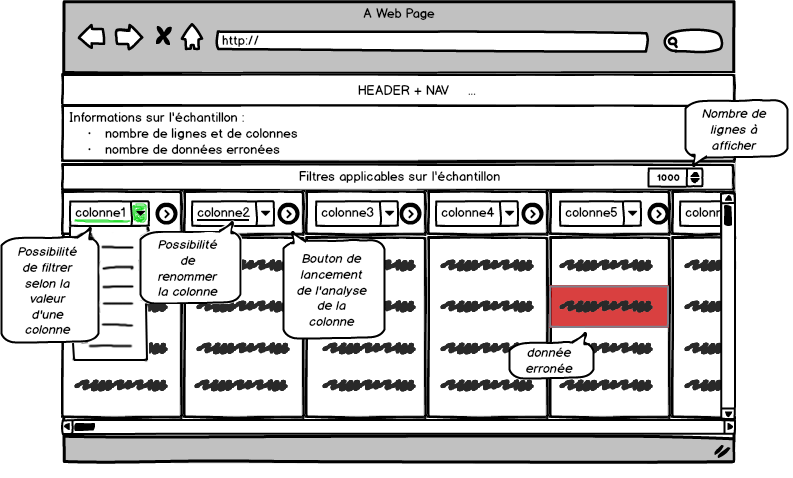
\includegraphics[scale=0.55]{fenetreEchantillons.png}\end{center}
			\begin{enumerate}
			
				\vspace{1em}\item Fonctionnalité d'affichage de l'échantillon :
					\begin{lstlisting}
						afficherEchantillon(lignesCSV, descCSV)
					\end{lstlisting}
					\underline{Paramètres :}
						\begin{description}[style=unboxed,leftmargin=0.2cm]
							\item\lstinline!lignesCSV! : \lstinline!list! - liste filtrée représentant les données du fichier CSV ligne par ligne.
							\item\lstinline!descCSV! : \lstinline!dict! - dictionnaire contenant 3 champs d'informations sur les colonnes du fichier CSV.
						\end{description}
					\underline{Retour :} sans retour (vide).\\
					\underline{Description :} cette fonction prend deux paramètres représentant l'échantillon pour en afficher le contenu sous forme de tableau.\\
					1 - Elle lit les champs \lstinline!"nom"! et \lstinline!"type"! du dictionnaire descriptif de l'échantillon et les affiche en en tête du tableau. \\
					2 - Elle lit simultanément, case par case, la liste des données l'échantillon filtré \lstinline!lignesCSV! et le champ \lstinline!"erreurs"! dictionnaire descriptif \lstinline!descCSV! et affiche la valeur de chaque donnée. Si une donnée est erronée, elle sera surlignée en rouge et un survol du curseur permettra d'afficher les informations sur cette erreur.
					
				\vspace{1em}\item Fonctionnalité de filtrage de l'échantillon selon la valeur exacte d'une colonne :
					\begin{lstlisting}
						filtreValeur(lignesCSV, nomColonne, valeurColonne)
					\end{lstlisting}
					\underline{Paramètres :}
						\begin{description}[style=unboxed,leftmargin=0.2cm]
							\item\lstinline!lignesCSV! : \lstinline!list! - liste représentant les données du fichier CSV en entier, ligne par ligne.
							\item\lstinline!nomColonne! : \lstinline!str! - nom de la colonne filtrante.
							\item\lstinline!valeurColonne! : type de la colonne - valeur de la colonne filtrante.
						\end{description}
					\underline{Retour :} une variable de type \lstinline!list! : une liste représentant les données du fichier CSV sur lesquelles le filtre a été appliqué.\\
					\underline{Description :} cette fonction prend en entrée la liste \lstinline!lignesCSV! représentant les données fichier CSV en entier, ligne par ligne. Elle renvoie ensuite une nouvelle liste filtrée représentant les données du fichier dont les valeurs de la colonne \lstinline!nomColonne! valent \lstinline!valeurColonne!.					
				
				\vspace{1em}\item Fonctionnalité de filtrage de l'échantillon selon une plage de valeurs d'une colonne :
					\begin{lstlisting}
						filtrePlageValeurs(lignesCSV, nomColonne, valeurColonneMin, ValeurColonneMax)
					\end{lstlisting}
					\underline{Paramètres :}
						\begin{description}[style=unboxed,leftmargin=0.2cm]
							\item\lstinline!lignesCSV! : \lstinline!list! - liste représentant les données du fichier CSV en entier, ligne par ligne.
							\item\lstinline!nomColonne! : \lstinline!str! - nom de la colonne filtrante.
							\item\lstinline!valeurColonneMin! : type de la colonne - valeur minimale de la colonne filtrante.
							\item\lstinline!valeurColonneMax! : type de la colonne - valeur maximale de la colonne filtrante.
						\end{description}
					\underline{Retour :} une variable de type \lstinline!list! : une liste représentant les données du fichier CSV sur lesquelles le filtre a été appliqué.\\
					\underline{Description :} cette fonction prend en entrée la liste \lstinline!lignesCSV! représentant les données fichier CSV en entier, ligne par ligne. Elle renvoie ensuite une nouvelle liste filtrée représentant les données du fichier dont les valeurs de la colonne \lstinline!nomColonne! sont comprises entre \lstinline!valeurColonneMin! et \lstinline!valeurColonneMax!.
									
				\vspace{1em}\item Fonctionnalité de filtrage de l'échantillon selon l'occurrence d'un arc du fichier CSV :
					\begin{lstlisting}
						filtreArc(lignesCSV, nomColonneDepart, nomColonneArrivee, valeurColonneDepart, ValeurColonneArrivee)
					\end{lstlisting}
					\underline{Paramètres :}
						\begin{description}[style=unboxed,leftmargin=0.2cm]
							\item\lstinline!lignesCSV! : \lstinline!list! - liste représentant les données du fichier CSV en entier, ligne par ligne.
							\item\lstinline!nomColonneDepart! : \lstinline!str! - nom de la colonne du nœud de départ l'arc.
							\item\lstinline!nomColonneArrivee! : \lstinline!str! - nom de la colonne du nœud d'arrivée de l'arc.
							\item\lstinline!valeurDepart! : type de la colonne - valeur de la colonne du nœud de départ l'arc.
							\item\lstinline!valeurArrivee! : type de la colonne - valeur de la colonne du nœud d'arrivée de l'arc.
						\end{description}
					\underline{Retour :} une variable de type \lstinline!list! : une liste représentant les données du fichier CSV sur lesquelles le filtre a été appliqué.\\
					\underline{Description :} cette fonction prend en entrée la liste \lstinline!lignesCSV! représentant les données fichier CSV en entier, ligne par ligne. Elle renvoie ensuite une nouvelle liste filtrée représentant les données du fichier dont les valeurs de la colonne \lstinline!nomColonneDepart! valent \lstinline!valeurDepart! et ceux de la colonne \lstinline!nomColonneArrivee! valent \lstinline!valeurArrivee!.
					
				\vspace{1em}\item Fonctionnalité de renommage de colonne :
					\begin{lstlisting}
						renommerColonne(descCSV, indiceColonne, nouveauNom)
					\end{lstlisting}
					\underline{Paramètres :}
						\begin{description}[style=unboxed,leftmargin=0.2cm]
							\item\lstinline!descCSV! : \lstinline!dict! - dictionnaire contenant 3 champs d'informations sur les colonnes du fichier CSV, à modifier.
							\item\lstinline!indiceColonne! : \lstinline!int! - numéro de la colonne à renommer.
							\item\lstinline!nouveauNom! : \lstinline!str! - nouveau nom à donner à la colonne.
						\end{description}
					\underline{Retour :} sans retour (vide).\\
					\underline{Description :} cette fonction prend en entrée le dictionnaire descriptif des colonnes \lstinline!descCSV!. Elle accède à la colonne d'indice \lstinline!indiceColonne! du champ \lstinline!"nom"! de ce dictionnaire, et remplace sa valeur par \lstinline!"nouveauNom"!.
					
				\vspace{1em}\item Fonctionnalité de choix de colonne à analyser :
					\begin{lstlisting}
						choixColonne(lignesCSV, indiceColonne)
					\end{lstlisting}
					\underline{Paramètres :}
						\begin{description}[style=unboxed,leftmargin=0.2cm]
							\item\lstinline!lignesCSV! : \lstinline!list! - liste représentant les données filtrées du fichier CSV en entier, ligne par ligne.
							\item\lstinline!indiceColonne! : \lstinline!int! - numéro de la colonne choisie.
						\end{description}
					\underline{Retour :} variable de type \lstinline!list! : liste simple contenant les données de la colonne choisie.\\
					\underline{Description :} cette fonction prend en entrée la liste \lstinline!lignesCSV! représentant les données filtrées du fichier CSV ligne par ligne. Elle crée une nouvelle liste pour y stocker une colonne unique. Elle parcourt le liste initiale ligne par ligne, et pour chaque ligne, elle stocke la valeur de la colonne d'indice \lstinline!indiceColonne! dans la nouvelle liste.
				
			\end{enumerate}
			
			
		\subsection{Module Fenêtre résultats ADD}
			Ce module est une fenêtre graphique web qui permet à l'utilisateur de consulter les résultats d'analyse des colonnes du fichier importé. La fenêtre résultats ADD est lancée avec la fonction \lstinline!fenetre_resultat_ADD()! du module Gestion des flux. Son contenu est disponible sur une page web et sera donc codé à l'aide de scripts JavaScript.
			\begin{enumerate}
				\item \underline{Aspect visuel :}\\
					\begin{center}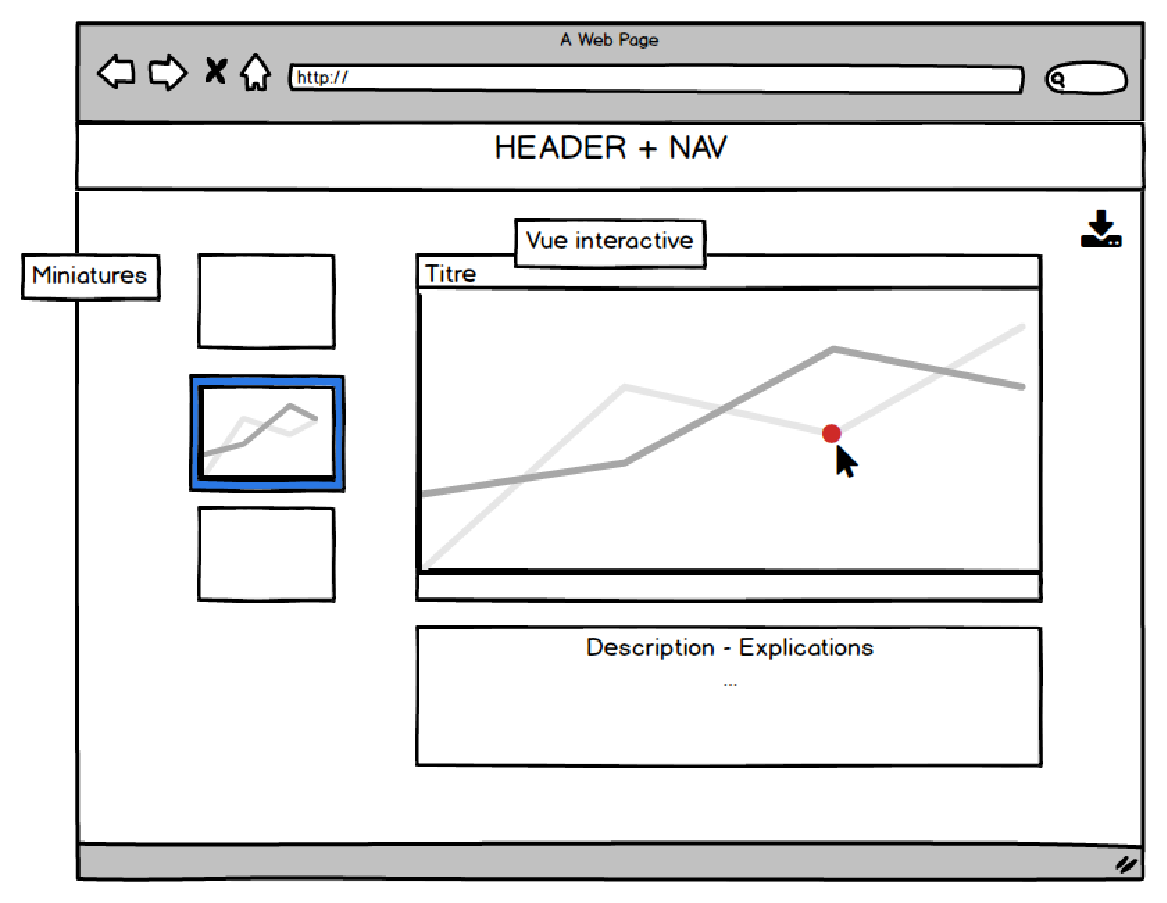
\includegraphics[scale=0.8]{FenetreADD.pdf}\end{center}
					Les résultats doivent se présenter de manière simple et sans surcharge. Les utilisateurs de ce produit doivent pouvoir prendre en main et comprendre les données sans pour autant être formés.
				\item \underline{Intéractions avec l'utilisateur :}\\
					\begin{itemize}
						\item Miniatures : Un clic sur une miniature permet de la faire basculer en vue précise.
						\item Vue précise : Un affichage interactif des valeurs rend la consultation plus intuitive et la charge de la vue plus légère. (une valeur non-demandée n'est pas affichée)
						\item Sauvegarde des résultats : Une simple icône de téléchargement permettra de lancer la sauvegarde des résultats en local. Cette sauvegarde passe par l'appel à la fonction du module Gestion des flux \lstinline!sauvegardeResultats()!.
					\end{itemize}
				\item \underline{Vues précises :}\\
					Ci-dessous, une liste des représentations graphiques disponibles, ainsi que le type d'analyse qui permet de les afficher :
					\begin{itemize}
						\item Histogramme : ADD qualitatives.
						\item Diagramme en secteur : ADD qualitatives.
						\item Série temporelle : ADD quantitatives.
						\item Diagramme en bâtons : Distribution des valeurs pour l'ADD quantitatives discrètes.
						\item Diagramme en escaliers : Distribution cumulative des valeurs pour l'ADD quantitatives discrètes.
						\item Courbe représentative : Distribution des valeurs pour l'ADD quantitatives continues.
						\item Courbe cumulative : Distribution cumulative des valeurs pour l'ADD quantitatives continues.
						\item Diagramme à moustaches : ADD quantitatives (discrète et conitnue).
					\end{itemize}
					Les données préparées pourles représentations graphiques sont aux formats \lstinline!.json! et \lstinline!.csv!. Les librairies c3js\footnote{http://c3js.org/} et d3js\footnote{https://d3js.org/} spécialisées dans les graphes et la présentation des données nous permettront d'obtenir ces représentations grpahiques.
			\end{enumerate}
	
	\section{Glossaire des types}
		Dans ce glossaire, on va préciser la définition des types des données qu'on a utilisé dans la description des fonctionnalités.
		\begin{itemize}
			\item \lstinline!TextIoWrapper! : classe représentant les flux de texte bufferisés (entrées/sorties de texte avec une sauvegarde dans une mémoire tampon). Elle permet donc de représenter les fichiers de texte brut en particulier. Elle définit des méthodes de manipulation de ces flux.
			\item \lstinline!str! : classe représentant des séquences de caractères (ou chaînes de caractères) en Python. Elle définit des méthodes de manipulation de ces chaînes.
			\item \lstinline!float! : classe représentant les nombres flottants à double précision en Python.
			\item \lstinline!list! : classe représentant des séquences de variables de type quelconque indexés par des entier. Elle définit des méthodes de manipulation de ces séquences.\\
				L'utilisation de ce type de données pour la manipulation des colonnes du fichier \lstinline!.csv! est préconisée car, tout d'abord, le type et les fonctions de manipulations sont disponibles directement avec Python, ensuite, ces listes sont implémentées sous forme de tableau ce qui garantie l'accès rapide à chacun de ses éléments, et enfin, leur taille maximale est définie par l'entier \lstinline!sys.maxsize!\footnote{https://docs.python.org/2/library/sys.html\#sys.maxsize} qui dépend des machines mais dépasse largement le million sur des PC bureautiques standards. Le million correspond à une borne maximale du nombre de lignes du fichier \lstinline!.csv! importé, la manipulation des listes peut donc se faire sans risque de crash mémoire.
			\item \lstinline!dict! : classe représentant des séquences de couple clés, variables (indexés par cette clé). Elle définit des méthodes de manipulation de ces séquences.
			\item \lstinline!.json! : (JavaScript Object Notation) format de données textuelles basé sur la notation des objets JavaScript. C'est un moyen simple d'accéder à des données car un flux JSON est une sérialisation (une traduction) d'un objet JavaScript.
			\item  \lstinline!Intervalle! : classe à implémenter
				\begin{lstlisting}
					class Intervalle:
				\end{lstlisting}
				\underline{Attributs :}
					\begin{itemize}
						\item \lstinline!borneInf : float! - limite inférieure de l'intervalle
						\item \lstinline!borneSup : float! limite supérieure de lintervalle
						\item \lstinline!infInclus : boolean! - vrai si l'intervalle est fermé à gauche
						\item \lstinline!supInclus : boolean! - vrai si l'intervalle est fermé à droite
						\item \lstinline!centre : float! - centre de l'intervalle calculé dans le constructeur
					\end{itemize}
				\underline{Méthodes :}
					\begin{itemize}
						\vspace{1em}\item
						\begin{lstlisting}
							__init__(self, borneInf, borneSup, infInclus, supInclus)
						\end{lstlisting}
						\underline{Description :} Constructeur
						
						\vspace{1em}\item
						\begin{lstlisting}
							contient(nombre)
						\end{lstlisting}
						\underline{Paramètres :}
							\begin{description}[style=unboxed,leftmargin=0.2cm]
								\item \lstinline!nombre : float!
							\end{description}
						\underline{Retour :} \lstinline!boolean!\\
						\underline{Description :} Renvoie vrai si \lstinline!nombre! est contenu dans l'intervalle, faux sinon.
					\end{itemize}
 		\end{itemize}
	
	\section*{Conclusion}
		Pour conclure, ce document décrit l'architecture de l'oeuvre en spécifiant les choix techniques qui ont été faits. Notre travail se résume en deux points. Tout d'abord Python va être le langage de programmation principal qui permet de gérer le calculet l'aspect web grâce aux librairies et aux frameworks disponibles. Ensuite, puisque nous codons une applet, JavaScript est l'outil le plus puissant pour assurer l'intéractivité de nos pages pour ainsi offrir une meilleure expérience à ses potentiels clients.\\
			
		Lors de la rédaction de ce document, plusieurs difficultés ont été rencontrées, notamment sur la spécification des aspects visuels du produit. En effet, ce produit étant une application web de traitement de données, on a été contraint d'adopter des outils de développement qui nous sont peu familiers : le langage Python et ses frameworks d'une part, et JavaScript d'autre part. Ces outils seront utilisés pour la réalisation des interfaces d'interaction avec l'utilisateur, ainsi que des rendus graphiques d'analyses. Par conséquent, il est possible que certaines de ces fonctionnalités s'avèrent non spécifiées. Mais aussi, l'intéractivité et le design des résultats nous pousse à tester les fonctionnalités sur une première version de l'applet pour pouvoir lancer une réflexion concrète sur le ressenti et l'expérience de l'utilisateur, ainsi les choix concernant les aspects graphiques sont les plus sujettes à des modifications.\\
		Néanmoins, et dans un cadre pédagogique, cette épreuve ne sera qu'enrichissante pour nous, non seulement sur le plan compétence, mais aussi expérience.
		
\end{document}
